\paragraph{}
This section details the proposed technique for adaptive scaled boundary finite element analysis. In comparison with the works in \cite{NME:NME439}, no stress recovery is required. This reduces the computational effort and leads to an efficient adaptive analysis. The error estimation is directly invoked from the scaled boundary finite element solutions.

%   ----    %
\subsection{Mesh Size}
\paragraph{}
The area of a subdomain will apparently influence the accuracy of the result.
Generally speaking, a larger subdomain tends to have a higher error.
The area of any polygon in fig.~\ref{adap_fig:ei_polygon} can be calculated as 

\begin{equation}
    S = \frac{1}{2}
        \sum_{k=1}
        \left(
            x_k y_{k+1} - x_{k+1} y_k
        \right)
\end{equation}

\begin{figure}[!h]
    \centering
    \scalebox{1}{
        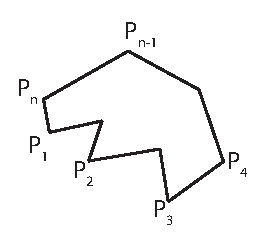
\includegraphics{adaptivity/images/adap_ei_polygon.eps}
    }
    \caption{A polygon with $n$ vertexes}
    \label{adap_fig:ei_polygon}
\end{figure}

%   ----    %
\subsection{Mesh Quality}
\paragraph{}
Mesh quality is another important factor that influence the accuracy.
In SBFEM, mesh quality is highly related to the minimal angle formed by the intersecting lines connected by scaling center and adjacent polygon vertexes.
An extremely smaller angel may raise numerical stability issue and hence decrease the accuracy of the result.

\begin{figure}[!ht]
    \begin{subfigure}[b]{0.5\linewidth}
        \centering
        \scalebox{1}{
            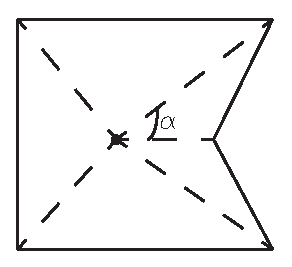
\includegraphics{adaptivity/images/adap_ei_mesh_quality_good.eps}
        }
        \caption{Acceptable}
    \end{subfigure}
    \begin{subfigure}[b]{0.5\linewidth}
        \centering
        \scalebox{1}{
            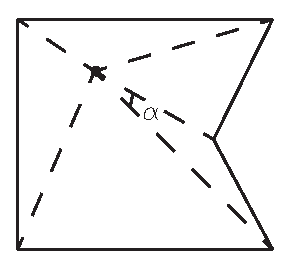
\includegraphics{adaptivity/images/adap_ei_mesh_quality_poor.eps}
        }
        \caption{Unacceptable}
    \end{subfigure}
    \label{adap_fig:ei_mesh_quality}
    \caption[Mesh quality in SBFEM]{Scaling center (
        \tikz[baseline=-0.5ex]\draw[black,fill=black] (0,0) circle (0.7ex);
    ), minimal angle $\alpha$}
\end{figure}

%   ----    %

\subsection{Eigenvalue in SBFEM}
\paragraph{}
From eq.~\ref{lr_eq:sbfem_displacement_field} ,the displacement SBFEM can be calculated as
\begin{equation}
    u(\xi) = c_1 \xi ^{-\lambda_1} \phi_u^1
            +c_2 \xi ^{-\lambda_2} \phi_u^2
            +\dots
\label{adap_eq:ei_terms}
\end{equation}
where $\phi_u^i$ stands for the eigenvector corresponding to the $i$th eigenvalue in the eigenvalue matrix $\Lambda^{n}$ in eq.~\ref{lr_eq:sbfem_eigen_decomp}.
The contribution of each mode is represented by every individual term in eq.~\ref{adap_eq:ei_terms} \cite{Deeks2002}.
On the other hand, after the displacement solution is calculated on the boundary nodes by eq.~\ref{lr_eq:sbfem_general_sol_disp} with $\xi=1$, displacement solution in circumferential direction then is interpolated by the help of the $p$-th order shape function $R(\eta)$ in eq.~\ref{lr_eq:sbfem_displacement_field}.
As a result, terms corresponding to the eigenvalue $\lambda_i \leq p$ can be exactly interpolated by the shape function.
These terms can be regarded as exact.
However, therms corresponding to the eigenvalue $\lambda_i > p$ indicates the shape function is not capable to interpolate the displacement exactly and thus shall be taken as error terms.
Consequently, displacement on the boundary $u(\xi=1)$ can be expressed with exact terms and approximation terms as followed
\begin{equation}
    u_b = u_e (\xi=1) + u_a(\xi=1)
\end{equation}
where the exact terms for the displacement on the boundary can be expressed as
\begin{equation}
    u_e (\xi=1) = \sum c_i \phi_u^i \text{   for all  } \lambda_i \leq p
\end{equation}
and similarly, the approximation terms can be written as
\begin{equation}
    u_a (\xi=1) = \sum c_i \phi_u^i \text{   for all  } \lambda_i > p
\end{equation}
Follow the same logic, nodal forces on the boundary can be expressed As
\begin{equation}
    \begin{aligned}
        q_b &= q_e(\xi=1) + q_a(\xi=1) \\
        q_e(\xi=1) &= \sum c_i \phi_q^i \text{   for all  } \lambda_i \leq p \\
        q_a(\xi=1) &= \sum c_j \phi_q^j \text{   for all  } \lambda_j > p \\
    \end{aligned}
\end{equation}
% energy
The energy can be calculated by the
\begin{equation}
    \begin{aligned}
        U &= \frac{1}{2} u_b^T q_b = U_e + U_a \\
        U_e &= u_e q_e\\
        U_a &= u_e q_a + u_a q_e + u_e q_e
    \end{aligned}
\end{equation}
The relative error for energy can be calculated as $\frac{U_a}{U}$ and the same logic for displacement and stress. 
\paragraph{}
In order to obtain satisfactory solutions within certain accuracy, the contribution of $U_a$ towards $U$ should be minimized and $U_a$ should also be distributed evenly to all cells. This is, in fact, similar to the relative energy norm error used in the literature \cite{NME:NME1620280411}.


\pagebreak